\documentclass[11pt,letterpaper]{article}

\usepackage[T1]{fontenc}
\usepackage[utf8]{inputenc}
\usepackage{graphicx}
\usepackage{geometry}
\usepackage{amsmath}
\usepackage{amssymb}
\usepackage{booktabs}
\usepackage{xcolor}
\usepackage{listings}
\usepackage[hyphens]{url}
\usepackage{natbib}
\usepackage{hyperref}

\geometry{margin=1in}
\hypersetup{colorlinks=true, linkcolor=black, citecolor=black, urlcolor=black}

% allow long code URLs in footnotes to break gracefully
\def\UrlBreaks{\do\/\do\-\do\_\do\.\do\=\do\?\do\&\do\:\do\a\do\b\do\c\do\d\do\e\do\f\do\g\do\h\do\i\do\j\do\k\do\l\do\m\do\n\do\o\do\p\do\q\do\r\do\s\do\t\do\u\do\v\do\w\do\x\do\y\do\z}
\Urlmuskip=0mu plus 1mu\relax

\title{Catching Silent Feature Absorption in Frozen Sparse Autoencoders:
Label-Free Localization, Averted-Cost Auditing, and a Cross-Dictionary
Absorber Catalog}

\author{Anonymous Authors}
\date{}

\begin{document}
\maketitle

\begin{abstract}
Single sparse-autoencoder (SAE) latents are unreliable units of analysis: feature absorption lets a specific child latent suppress a more general parent, leaving the parent with silent recall holes on exactly the sub-contexts the child covers. The natural fix---grouping latents into a cluster-level unit---did not pay off in our experiments: multi-member grouping is inert, tying a single most-precise latent on every edit and matching weak baselines on classification. We instead deliver \emph{label-free single-specialist localization}: anchor on the highest-recall parent latent, read its recall hole to name an under-served sub-context with no sub-context labels, and precision-select the single absorber that marginal-attribution selection silently drops. Three results turn this operator into a build-on capability. (1) \textbf{Averted cost}: on a compact classifier and steering handle selected by the standard SCR/TPP marginal-attribution practice, absorption silently breaks the absorbed slice (Georgia country-recall $0.107$ vs.\ $0.969$ on siblings; the absorber sits at attribution rank $42$, outside any compact top-$N$, and the field's decoder-cosine proxy is blind to it); our shipped label-free screen flags the hole and names the absorber, and a two-member repair unit recovers the classifier to $\approx1.0$ ($+0.89$, CI excludes $0$) and the steer by $+5.74$, matching a hole-free dense probe while staying sparse. (2) \textbf{Genuine cross-deployment transfer}: a fixed absorber id beats a fresh $n$-label dense gate at zero deployment labels on $4/5$ sub-contexts. (3) A \textbf{$1344$-row absorber catalog} over a four-SAE Gemma Scope suite, showing absorption is far more prevalent at the earlier layer. We are explicit about the ceiling: no SAE unit out-classifies a dense probe, the edit is matched by a fair labeled gate, and the structure is homograph/named-entity-confined ($6/110$ tokens). All experiments run on a single GPU over public, frozen SAEs.
\end{abstract}

\section{Introduction}
\label{sec:intro}

Sparse autoencoders (SAEs) decompose the activations of large language models (LLMs) into a dictionary of sparsely-activating latents intended to be interpretable, monosemantic units of analysis \citep{Cunningham2023, Bricken2023, Templeton2024}. The operational promise is that a latent tracking a human concept can be read off as a classifier, flipped as a steering knob, or compared across model variants. Public SAE suites such as Gemma Scope \citep{Lieberum2024} expose millions of latents over open models, making this the practical interface for safety-relevant interpretability and the substrate our work operates on.

That promise is undercut by a documented fact: \emph{single SAE latents are not reliable units} \citep{Leask2025}. Two failure modes recur. \emph{Feature splitting} fragments one concept across many latents. \emph{Feature absorption} is more insidious: a more specific child latent suppresses the firing of a more general parent, leaving the parent with unpredictable holes on exactly the sub-contexts the child covers; parent and child become \emph{mutually exclusive in firing} \citep{Chanin2024}. On concrete tasks the cost is stark---difference-of-means probes are the strongest concept detectors and raw-latent SAE methods are uncompetitive \citep{Wu2025, Kantamneni2025}---while standardized suites that quantify absorption are themselves of contested reliability \citep{Karvonen2025, Chanin2026}.

Why is this hard, and why is it not already solved post-hoc? Absorption defeats the obvious instruments \emph{by construction}. Every observational grouping signal---which latents fire together \citep{ONeill2024, Deng2025}, or which decoder directions point alike---must fail, because the parent and its absorbing child are firing-disjoint (firing-Jaccard $<0.05$) and their decoders need not be cosine-similar \citep{Chanin2024}. The standard \emph{supervised} remedy---ranking latents by marginal causal effect on a concept probe and ablating the top-$N$ \citep{Karvonen2024, Marks2024}---is no better: an absorber that fires only in a narrow sub-context has a small broad-distribution class-mean gap, hence a small marginal attribution, hence falls below any compact top-$N$ cut and is silently dropped. Architectural remedies---Matryoshka \citep{Bussmann2025}, hierarchical \citep{Muchane2025}, and subspace-aware SAEs \citep{Dalili2026}---all \emph{retrain} the SAE and do not help a practitioner holding a frozen public SAE.

The natural fix for an unreliable single latent is to group several latents into a cluster-level unit, and the goal we set was exactly that. We report, as a primary finding, that the clustering hypothesis did not pay off (\S\ref{sec:nulls}): multi-member grouping is \emph{inert}---replacing the anchored cluster with the single most precise latent ties it on every edit ($0/8$ cases where the machinery adds value), ablating the full unit lowers retained utility, and a correlation-community track ties weak baselines for classification \footnote{Code: \url{https://github.com/AMGrobelnik/ai-invention-7ee30c-catching-silent-feature-absorption-in-fr/tree/main/round-8/experiment-1}}. The durable object is not a cluster but a single \emph{label-free-localized specialist} together with a minimal two-member \emph{parent$\oplus$absorber} repair unit.

Our matched instrument is \textbf{label-free single-specialist localization} (\S\ref{sec:method}): given only content-flip pairs, anchor on the highest-recall parent latent, read its recall \emph{hole} to name an under-served sub-context with no sub-context labels, and precision-select the single latent covering it---the very absorber that marginal attribution drops. From this one operator we build a shipped label-free \emph{screen}, an auditable feature-level knowledge graph (KG), a measured repair unit, and a cross-dictionary \emph{catalog}.

\begin{figure*}[!t]
  \centering
  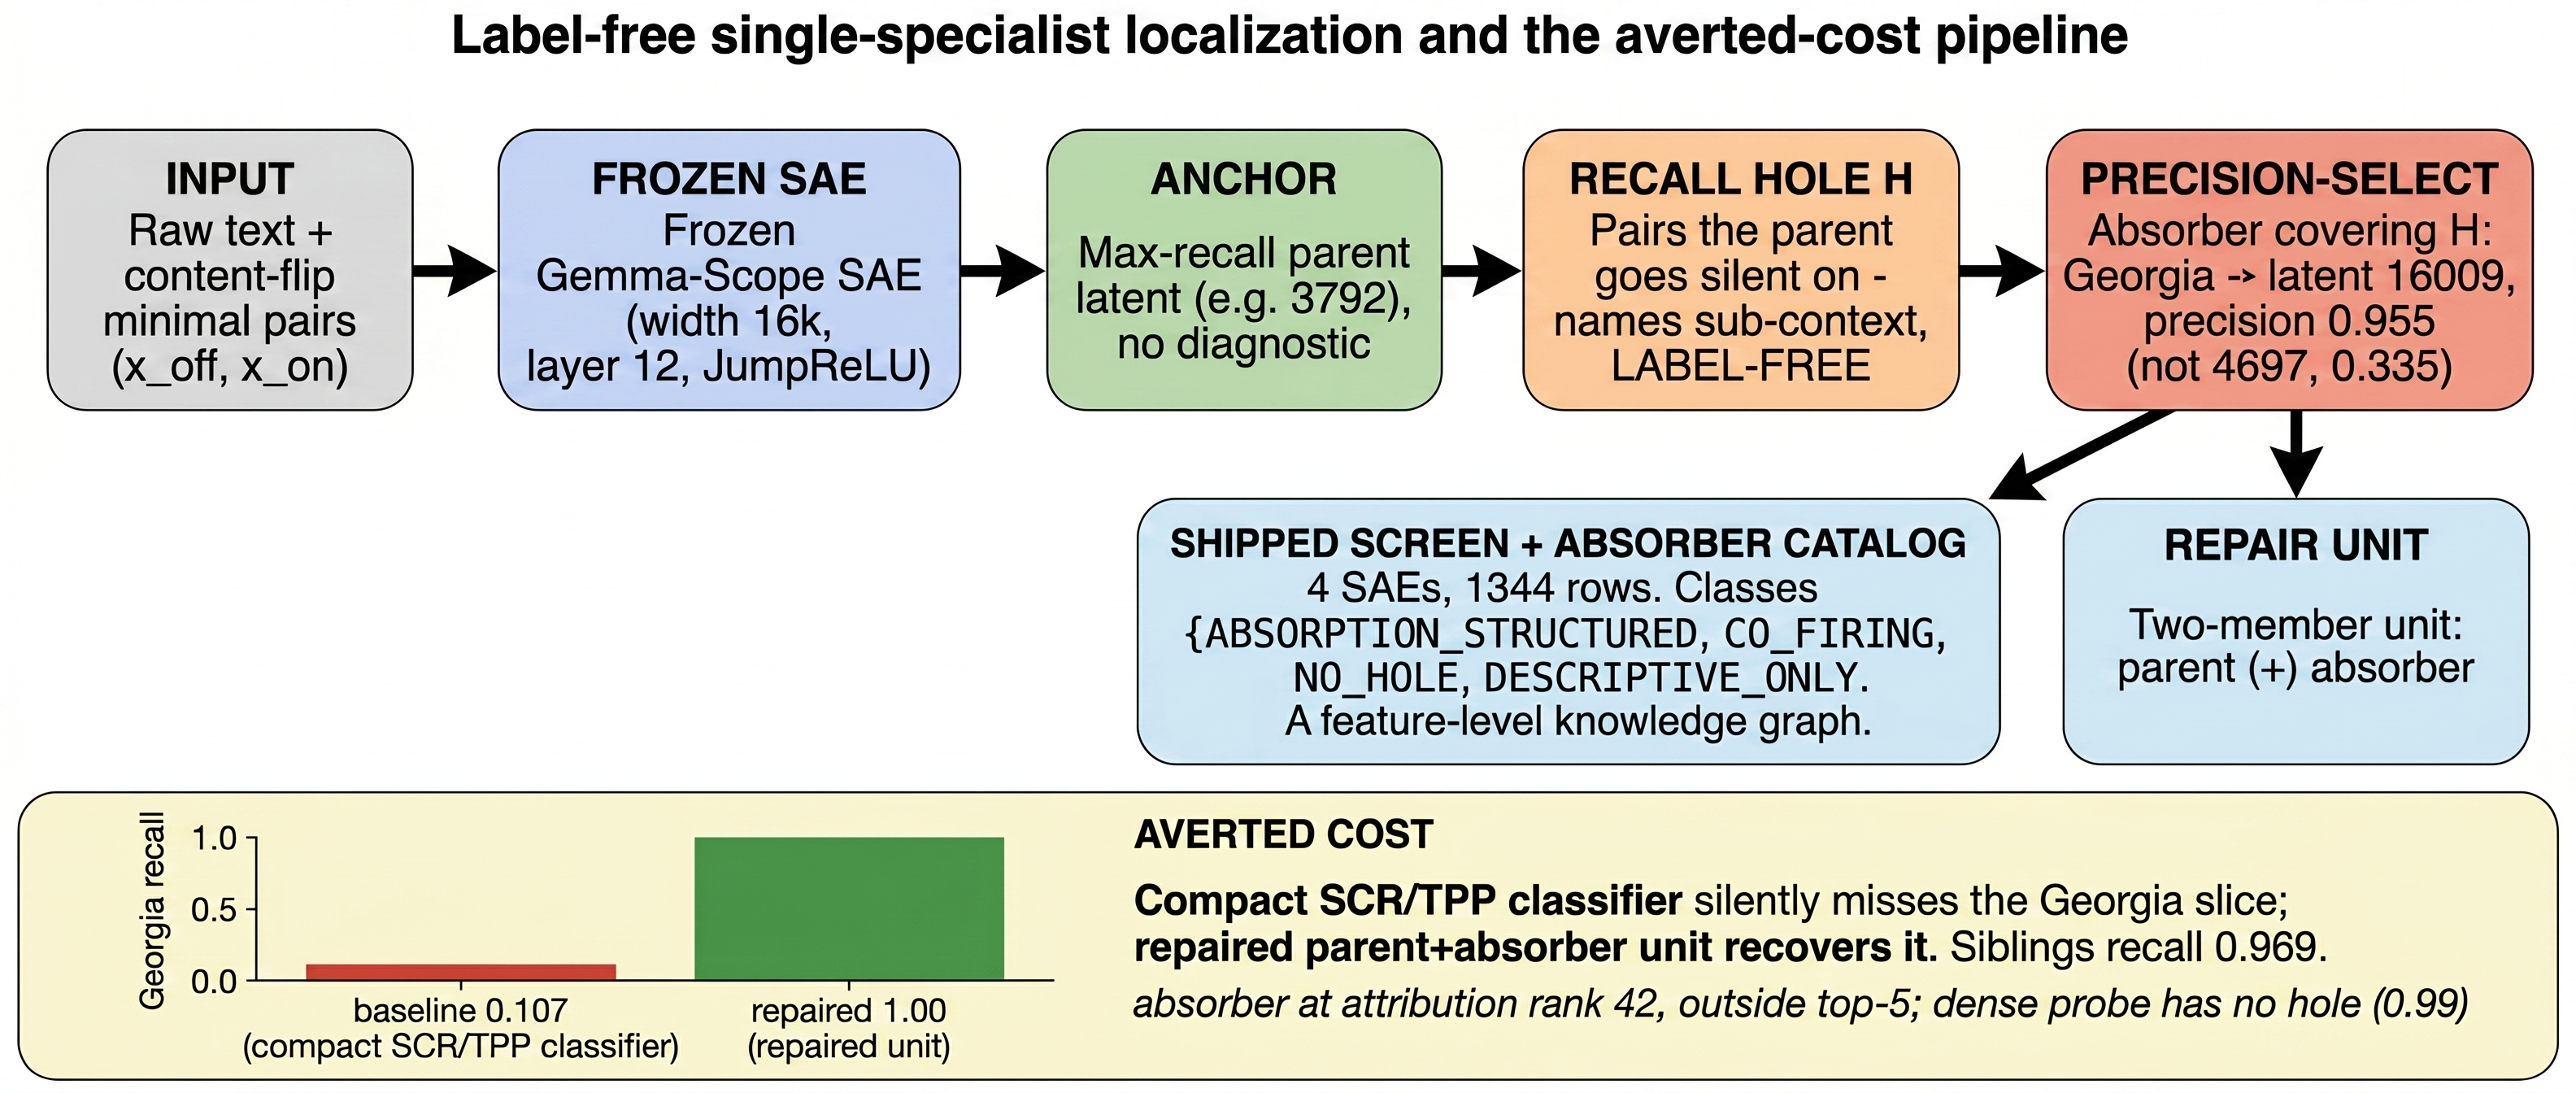
\includegraphics[width=\textwidth,height=0.45\textheight,keepaspectratio]{figures/fig1_v0.jpg}
  \caption{From a frozen SAE and content-flip pairs, anchor on the highest-recall parent latent, read its recall hole to name an under-served sub-context label-free, and precision-select the single absorber marginal attribution drops. The operator yields a shipped screen, a cross-dictionary absorber catalog (a feature-level knowledge graph), and a two-member parent$\oplus$absorber repair unit. Bottom: a compact SCR/TPP classifier silently misses the Georgia slice (recall 0.107); the repaired unit recovers it to 1.0.}
  \label{fig:pipeline}
\end{figure*}

The reposition lets us deliver three demonstrated, positive results while being explicit about a narrow ceiling.

\paragraph{(1) Averted-cost auditing turns the screen into a capability (\S\ref{sec:averted}).} A practitioner who ships a compact, human-auditable classifier or steering handle selected by the standard SCR/TPP marginal-attribution practice silently fails on the absorbed slice (Georgia country-recall $0.107$ vs.\ $0.969$ on siblings); standard tooling misses it (the absorber is at attribution rank $42$, outside any compact top-$N$, and the field's decoder-cosine oracle is blind to it); our shipped screen catches it label-free and names the absorber; and adding the named absorber as a two-member unit repairs the classifier to $\approx 1.0$ ($+0.89$, CI excludes $0$) and the steer by $+5.74$, matching a dense probe that has no hole \footnote{Code: \url{https://github.com/AMGrobelnik/ai-invention-7ee30c-catching-silent-feature-absorption-in-fr/tree/main/round-10/experiment-1}}.

\paragraph{(2) Genuine cross-deployment where-to-gate transfer (\S\ref{sec:transfer}).} An absorber id discovered once on deployment $A$, applied with \emph{zero} new labels to a disjoint deployment $B$, beats a fresh $n$-label dense gate on $4/5$ sub-contexts (Georgia/United States/Amazon on a held-out corpus split, the spelling case ``\texttt{large}'' on a carrier shift), with Jordan an honest no-transfer case \footnote{Code: \url{https://github.com/AMGrobelnik/ai-invention-7ee30c-catching-silent-feature-absorption-in-fr/tree/main/round-10/experiment-3}}.

\paragraph{(3) An auditable spine and a published catalog (\S\ref{sec:spine}, \S\ref{sec:catalog}).} The KG-named absorber recovers the parent's recall hole over the two informative label-free selectors at FDR$\le0.05$ on $16/24$ holes; the localization is auditable (member-labeling agreement $0.730$ vs.\ a $0.096$ null) and replicates on a $4\times$-wider SAE \footnote{Code: \url{https://github.com/AMGrobelnik/ai-invention-7ee30c-catching-silent-feature-absorption-in-fr/tree/main/round-9/experiment-3}}. We ship a label-free absorber catalog over a four-SAE Gemma Scope suite that reproduces our screen bit-exactly and maps where absorption hides across dictionaries.

\paragraph{Honest ceiling.} No SAE unit out-classifies a dense probe (\S\ref{sec:nulls}); the edit, as an edit, is matched by a fair labeled gate \citep{Lee2024, Zhang2026}; and absorption is homograph/named-entity-confined ($6/110$ eligible polysemous tokens). We report these as findings, not as future work.

\paragraph{Summary of contributions.}
\begin{itemize}
\item \textbf{An averted-cost capability} (\S\ref{sec:averted}): the first end-to-end demonstration that absorption silently breaks a compact SAE-latent classifier/steerer the standard practice ships, that a label-free screen catches it where standard tooling does not, and that a two-member repair unit fixes it with a bootstrap-CI-measured benefit---the answer to ``why build on this.''
\item \textbf{A genuine, de-inflated where-to-gate saving} (\S\ref{sec:transfer}): a fixed absorber id transfers zero-label to a disjoint deployment and beats an $n$-label dense gate on $4/5$ sub-contexts, with a reported break-even $K^\star$ and one honest no-transfer case, removing the circularity of a prior same-fold comparison.
\item \textbf{A re-controlled localization spine} (\S\ref{sec:spine}): the absorber beats the two \emph{informative} label-free selectors on $16/24$ holes (the parent-argmax controls are reported only as vacuous-by-construction confirmations), with a selection-independent behavioral-KL metric, LLM-auditable members, and $4\times$-width replication.
\item \textbf{A label-free screen and cross-dictionary catalog} (\S\ref{sec:catalog}): a shipped tool plus a $1344$-row absorber catalog over four public SAEs (a feature-level knowledge graph), with the confinement boundary ($6/110$ eligible tokens; demographic attributes never structured).
\item \textbf{Honestly-reported nulls} (\S\ref{sec:nulls}): clustering inert; no dense-probe out-classification; steering surgical on $2/5$ letters; model-diffing a confound-bounded $+0.000$ null; the edit matched by a fair labeled gate.
\end{itemize}

\section{Related Work}
\label{sec:related}

\paragraph{Unreliable single latents.} Sparse dictionary learning yields interpretable features \citep{Cunningham2023, Bricken2023, Templeton2024, Lieberum2024}, but individual latents are not canonical units \citep{Leask2025}. \citet{Chanin2024} introduce and quantify \emph{absorption}---a specific child suppresses a general parent, demonstrated on first-letter spelling---and \citet{Chanin2025} give the two-sided width law (absorption worsens as the SAE widens). Benchmarks make the cost concrete---difference-of-means is strongest and raw-latent SAE methods are uncompetitive \citep{Wu2025, Kantamneni2025}---and SAEBench reports that absorption scores worsen with dictionary size \citep{Karvonen2025}. Crucially, the field's own reliability proxies are contested: \citet{Chanin2026} find that the SCR and TPP metrics ``fail multiple lenses\ldots should not be used,'' motivating a task-grounded, label-free, oracle-validated screen (\S\ref{sec:catalog}). \citet{Minegishi2025} argue SAE quality is fundamentally a question of polysemous-word representation, predicting the lexical shape of our confinement finding.

\paragraph{Grouping and supervised selection.} Prior grouping is observational: co-activation feature families \citep{ONeill2024}, sparse coactivation modules \citep{Deng2025}, and the closest feature-level KG \citep{Winnicki2026}, which builds edges from corpus co-occurrence and transcoder geometry. By construction such edges cannot express our central relation---a parent anchor joined to a specialist that is \emph{firing-disjoint} (low co-occurrence) and decoder-orthogonal (Georgia decoder-cosine $\approx 0.01$); our catalog edges are interventional firing-signature absorption structure, complementary to the observational view. SHIFT and the SCR/TPP family rank individual latents by marginal causal effect and ablate the top-$N$ \citep{Marks2024, Karvonen2024}; an absorber's small broad-distribution class-mean gap drops it below the threshold by construction---the silent failure our averted-cost scenario exploits (\S\ref{sec:averted}).

\paragraph{The absorption diagnostic and our delta.} \citet{Chanin2024} provide a \emph{supervised, spelling-bound} diagnostic: a logistic probe on ground-truth first-letter labels locates the parent, an ablation on the first-letter logit plus a probe-projection test locates the absorber (decoder-cosine threshold $0.025$). Our delta is to make discovery \emph{label-free, training-free, and form-free}: the parent is anchored by content-response recall, its recall hole names the sub-context (no logit, no sub-context labels), and the absorber is chosen by firing-precision; the form-free probe$+$ablation diagnostic only \emph{scores} already-formed KG edges, never forms them. We run it on homograph/numeric/named-entity hierarchies the diagnostic was never applied to, and we show the supervised decoder-cosine proxy is blind to the very Georgia absorber our screen catches ($\textrm{cos}\approx 0.012<0.025$).

\paragraph{Gating is prior art; the value is where-to-gate.} Gating an edit by a sparse/threshold detector is established prior art: CAST applies a steering vector when a learned condition vector matches \citep{Lee2024}; GSS publishes essentially our footprint control's operator with probe and steer optimized on labeled sequences \citep{Zhang2026}; GUARD-IT routes through a similarity gate over labeled clusters \citep{Turani2026}; SADI builds a per-input mask from contrastive pairs \citep{Wang2024}. In all of these the gate is \emph{supervised}. The SAE-specific value is the label-free discovery of \emph{where} to gate \citep{Peng2025}, whose net saving \S\ref{sec:transfer} demonstrates under genuine cross-deployment transfer. We measure quality versus the number of sub-context labels as an empirical loss-data curve \citep{Whitney2020} against the provably-strong difference-of-means direction \citep{Im2025}, whose supervised steering directions are dataset-dependent and brittle \citep{Tan2024}; active learning reduces but does not remove the label cost \citep{Rauch2025, Cho2022, Chatzoudis2025}.

\paragraph{Selection, robustness, and dense comparators.} \emph{Which} precise feature is selected drives clean edits \citep{Arad2025, Chalnev2024, Duan2026}; ``specificity'' is exactly a sharp conditional gate \citep{Templeton2024}---our concentration-not-absorption finding sits in this line (\S\ref{sec:nulls}). SAE unlearning has side-effects $\ge$ fine-tuning for whole topics \citep{Farrell2024}; a labeled dense direction can be erased while preserving utility \citep{Belrose2023, KarvonenMarks2025, He2025, Ashuach2025}, and we map outcomes onto the forget/retain/fluency triad \citep{Li2024, Shi2024}. SAE debiasing edits \emph{whole} bias-correlated features \citep{Sasse2024, Xu2025}; the closest near-miss steers a single race-correlated latent that \emph{co-fires} and concedes SAE steering is ``of marginal utility'' \citep{Ahsan2025}, corroborating our homograph-confined safety null. SAE features classify and transfer under pooling \citep{Gallifant2025}, which does not contradict our single-latent localization-not-classification claim. The robustness framing engages label-free worst-group robustness \citep{Sagawa2019, Liu2021, Sohoni2020, Creager2020, Nam2020, Rudner2024}, which infers groups over \emph{examples} and retrains; we group features and never retrain. Cross-field instruments---maximum coverage \citep{Nemhauser1978, Feige1998}, differential co-expression \citep{Tesson2010, Zhang2005}, Leiden \citep{Traag2018}---are motivation; minimal-pair sources are CAD \citep{Kaushik2019}, CEBaB \citep{Abraham2022}, ParaDetox \citep{Logacheva2022}, civil\_comments \citep{Borkan2019}, bias\_in\_bios \citep{DeArteaga2019}; surface invariance draws on \citep{Belrose2023, Veitch2021}; the closest counterfactual-clustering template is CDLC in vision \citep{Varshney2025}.

\section{Label-Free Single-Specialist Localization}
\label{sec:method}

One training-free operator---anchor, read the recall hole, precision-select the absorber---surfaces the specialist that marginal attribution drops, using no sub-context labels.

\paragraph{Preliminaries.} The frozen SAE has latents $l\in\{1,\dots,L\}$ with encoder activation $a_l(x)$; a latent \emph{fires} on $x$ iff $a_l(x)>0$ (Gemma Scope uses a JumpReLU \citep{Lieberum2024}). For a concept $c$ we are given \emph{content-flip minimal pairs} $(x_{\text{off}},x_{\text{on}})$, the supervision every matched baseline consumes; the method uses \emph{no} per-sub-context labels and \emph{no} absorption-specific oracle. The primary run encodes at one residual-stream site (\texttt{gemma-2-2b}, layer 12, width 16k canonical; $d_{\text{model}}=2304$, gating cosine $0.919$); \S\ref{sec:catalog} re-runs at width 65k and layer 9.

\paragraph{The operator.} \textbf{(i) Content-response cover sets.} For latent $l$ and pair $p$, the content-response is $r_l(p)=a_l(x_{\text{on}})-a_l(x_{\text{off}})$; the cover set $C_l$ is the pairs whose flip $l$ tracks reliably ($r_l(p)>\tau_{\text{resp}}$, $a_l(x_{\text{on}})>0$) and precisely (firing-precision $\ge0.7$ on its own support). Because absorbers fire on a handful of words, eligibility is cover-based, not mean-over-pairs. \textbf{(ii) Anchor.} $l^{*}=\arg\max_l|C_l|$, the highest-recall parent candidate, chosen using only the pairs and \emph{not} the absorption diagnostic; an unsupervised firing-floor step requires the anchor to fire on held-out corpus above $5\%$. \textbf{(iii) Hole.} $H=P\setminus C_{\text{anchor}}$, the pairs the parent goes silent on---the recall hole that names the under-served sub-context, label-free. \textbf{(iv) Precision-select.} over latents covering $H$, choose by held-out per-sub-context firing-precision the specialist (Georgia selects latent $16009$ at precision $0.955$, not $4697$ at $0.335$), subject to firing-Jaccard $<0.1$ and a bootstrap-CI-positive coverage gain.

\paragraph{Non-circular diagnostic and auditable graph.} Specialization edges are \emph{scored}, never formed, by the form-free probe-projection of \citet{Chanin2024} (SAEBench \texttt{absorption\_fraction}), with the parent probe trained on data disjoint from grouping. Each admitted unit is emitted with logit-lens tokens, top conditioning contexts, and a directed anchor$\to$absorber edge---a feature-level KG. The discovery is \emph{amortized and transferable label-free}: an absorber is named once and reused, consuming zero per-sub-context labels (the distinction that powers \S\ref{sec:transfer}).

\paragraph{The shipped screen.} The same firing signature classifies any candidate token as \textsc{Absorption-Structured}, \textsc{Co-Firing}, \textsc{No-Hole}, or \textsc{Descriptive-Only}---parent recall-hole $>0.5$, firing-disjoint absorber (Jaccard $<0.1$), absorber precision $\ge0.7$, hole-coverage gain CI $>0$, and $\ge150$ eligible for the strict (inferential) gate---using \emph{no} diagnostic probe and \emph{no} sub-context labels. \texttt{screen.py} is the practitioner deliverable that \S\ref{sec:averted} and \S\ref{sec:catalog} are built on.

\paragraph{Operators, defined once.} Table~\ref{tab:ops} fixes the six edit/gate operators used throughout. The single SAE-specific object is \textsc{KG-Abl}: ablate the named absorber, $h\leftarrow h-\lambda z_l W_{\text{dec}}[l]$, gated by the latent's own sparse firing, using \emph{zero} sub-context labels. \textsc{Repair} instead adds the absorber to the suppressed parent to recover its recall hole---the two-member unit of \S\ref{sec:averted}.

\begin{table}[t]
\centering\small
\caption{The six operators, defined once. ``labels'' = number of \emph{per-sub-context} labels required at deploy. Retain collateral is on \texttt{large} at matched meaningful forget (code: \protect\url{https://github.com/AMGrobelnik/ai-invention-7ee30c-catching-silent-feature-absorption-in-fr/tree/main/round-9/evaluation-1}). \textsc{KG-Abl} is the only label-free SAE handle; \textsc{Max-Prec} is the ablation showing set-cover discovery is inert; \textsc{Dense-Whole} is the disowned strawman that is the selectivity denominator in \S\ref{sec:spine}.}
\label{tab:ops}
\begin{tabular}{lllc}
\toprule
Operator & what it does & labels & retain collat. \\
\midrule
\textsc{KG-Abl} (handle) & ablate named absorber, gated by its own firing & $0$ & $5.1\times10^{-5}$ \\
\textsc{Dense-Sub} (lead) & ungated diff-of-means erasure of $u_{\text{sub}}$ & $n$ & $2.1\times10^{-2}$ \\
\textsc{Dense-Sub-Fair} & erase $u_{\text{sub}}$ where logistic $d_{\text{sub}}$ fires, $\beta\le1$ & $n$ & $2.8\times10^{-6}$ \\
\textsc{Dense-Sub-Foot} & footprint-matched magnitude gate (demoted) & $n$ & $2.9\times10^{-1}$ \\
\textsc{Max-Prec} & single most-precise latent (no anchoring) & $0$ & $5.1\times10^{-5}$ \\
\textsc{Dense-Whole} & whole-parent erasure (strawman) & $n$ & $2.6$ \\
\bottomrule
\end{tabular}
\end{table}

\section{Testbeds and Protocol}
\label{sec:setup}

We built seven frozen, schema-standardized families, all pure text/data, so absorption presence is an empirical question for the SAE run: first-letter spelling ($17{,}180$ examples) \footnote{Code: \url{https://github.com/AMGrobelnik/ai-invention-7ee30c-catching-silent-feature-absorption-in-fr/tree/main/round-1/dataset-1}}; numeric/taxonomic ($24{,}128$) \footnote{Code: \url{https://github.com/AMGrobelnik/ai-invention-7ee30c-catching-silent-feature-absorption-in-fr/tree/main/round-1/dataset-2}}; toxicity ($37{,}707$) \footnote{Code: \url{https://github.com/AMGrobelnik/ai-invention-7ee30c-catching-silent-feature-absorption-in-fr/tree/main/round-1/dataset-3}}; a sentiment/aspect/boundary-null support family ($30{,}739$) \footnote{Code: \url{https://github.com/AMGrobelnik/ai-invention-7ee30c-catching-silent-feature-absorption-in-fr/tree/main/round-1/dataset-4}}; a homograph-entity testbed \footnote{Code: \url{https://github.com/AMGrobelnik/ai-invention-7ee30c-catching-silent-feature-absorption-in-fr/tree/main/round-5/dataset-1}}; and a safety-identity testbed ($36{,}448$) \footnote{Code: \url{https://github.com/AMGrobelnik/ai-invention-7ee30c-catching-silent-feature-absorption-in-fr/tree/main/round-6/dataset-1}}. Baselines span raw latents, the SCR/TPP marginal-attribution selection (the standard practice), dense difference-of-means probes, and four label-free selectors. The primary inferential object is a per-concept paired or two-sample bootstrap of an AUC, recall, or outcome difference ($B{=}10{,}000$, resampling pairs/prompts as clusters), with FDR or Holm--Bonferroni control across headline claims; any edit-quality claim additionally requires a second different-family LLM judge to exclude $0$. Gemma Scope is loaded from \texttt{params.npz} (canonical \texttt{layer\_12/}\allowbreak\texttt{width\_16k}, JumpReLU, gating cosine $0.919$); encoding pins are in Appendix~\ref{sec:appendix}.

\section{Averted-Cost Auditing: Absorption Silently Breaks Compact Units}
\label{sec:averted}

On a downstream artifact a practitioner would actually ship, absorption silently breaks the absorbed slice, standard practice misses it, the shipped screen catches it label-free, and a two-member repair unit fixes it with a bootstrap-CI-measured benefit. Overall verdict: averted cost demonstrated on $3/4$ arms (the fourth is an honest, conservative abstention).

\paragraph{Setup.} We ship two artifacts built on frozen Gemma-Scope latents: a parent-concept \emph{classifier} (a logistic head on the pooled top-$N$ latents) and a parent-concept \emph{steering} handle, both selected by SCR/TPP marginal attribution ($|$probe weight$|\times$mean positive activation), the standard raw-latent practice \citep{Karvonen2024, Marks2024}. The compact, human-auditable selection size the goal asks for is $k\le5$; the headline is $N{=}5$, with the full curve $N\in\{1,2,5,10,20\}$ reported.

\begin{figure*}[!t]
  \centering
  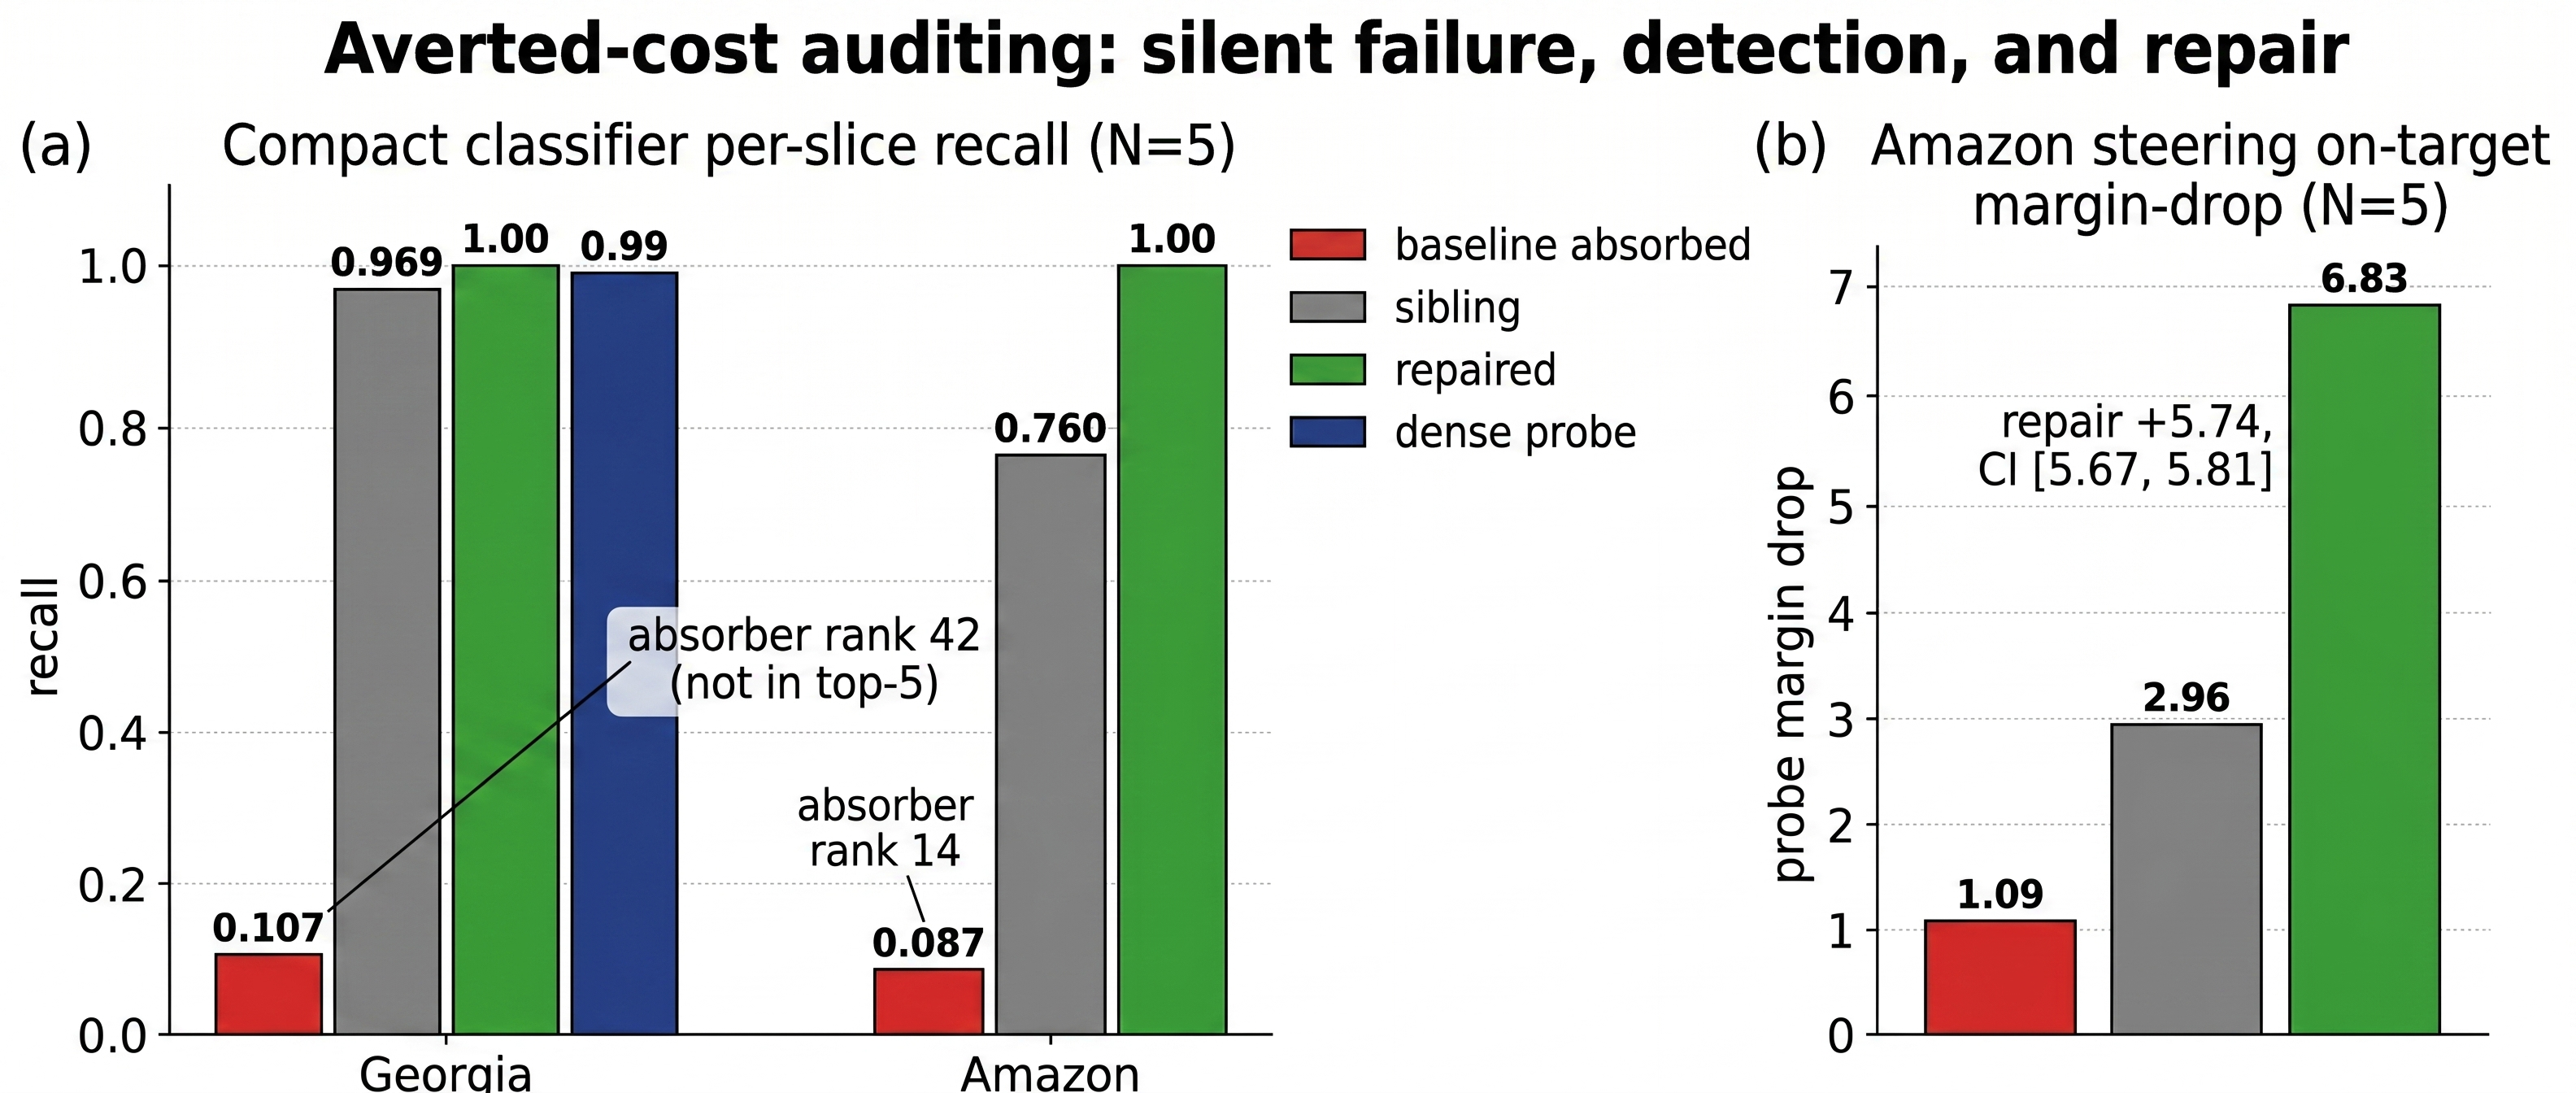
\includegraphics[width=\textwidth,height=0.45\textheight,keepaspectratio]{figures/fig2_v0.jpg}
  \caption{On compact (N=5) SCR/TPP-selected units, absorption silently breaks the absorbed slice; the named-absorber repair recovers it. Left: per-slice recall for the Georgia (country) and Amazon (org) classifiers. Right: Amazon steering on-target margin-drop. The dense probe has no hole (Georgia 0.99). All gap/repair CIs (B=10,000) exclude 0.}
  \label{fig:averted}
\end{figure*}

\paragraph{(a) Silent failure.} At compact sizes the absorbed slice is silently missed (Table~\ref{tab:averted}): the Georgia country-recall is $0.107$ vs.\ $0.969$ on the $20$ sibling countries (gap $+0.862$, CI $[0.809,0.910]$); the Amazon org-recall is $0.087$ vs.\ $0.760$ (gap $+0.673$); the Amazon steering on-target margin-drop is $1.09$ vs.\ $2.96$ on siblings (gap $+1.87$). \textbf{(b) Standard practice misses it.} The absorber is buried deep in the SCR/TPP ranking---Georgia's latent $16009$ at rank $42$, Amazon's $6846$ at rank $14$---far below any compact top-$N$. And the form-free decoder-projection oracle scores Georgia \emph{clean} (decoder-cosine $-0.024$, $|\cdot|<0.025$, does not corroborate), exactly because Georgia's absorber is near-orthogonal to the generic ``country'' direction; it does corroborate the lexical Amazon case (cosine $0.116$). \textbf{(c) The screen catches it.} The shipped label-free screen flags \textsc{Absorption-Structured} (Georgia recall-hole $0.733$, firing-Jaccard $0.013$, precision $0.974$; Amazon $0.62$/$0.043$/$0.993$) and names the absorber with zero sub-context labels. \textbf{(d) The repair.} Adding the named absorber as a two-member parent$\oplus$absorber unit lifts the Georgia classifier to recall $1.0$ (KG$-$baseline $+0.893$, CI $[0.84,0.94]$), the Amazon classifier to $1.0$ ($+0.913$), and the Amazon steer on-target to $6.83$ ($+5.74$, CI $[5.67,5.81]$), with no sibling collateral.

\begin{table}[t]
\centering\small
\caption{Averted-cost auditing ($N{=}5$, the compact auditable size). Absorption silently breaks the absorbed slice; the absorber sits outside the compact top-$N$ (its attribution rank); the screen flags it; the named-absorber repair recovers it. The non-SAE dense probe has \emph{no} hole, so the hole is an SAE-selection artifact and the repair is specific to it. All gaps/repairs have $B{=}10{,}000$ bootstrap CIs excluding $0$.}
\label{tab:averted}
\begin{tabular}{llccccc}
\toprule
Arm & metric & absorbed & sibling & attr.\ rank & repaired & dense \\
\midrule
Georgia (clf) & recall & $0.107$ & $0.969$ & $42$ & $1.00$ & $0.99$ \\
Amazon (clf) & recall & $0.087$ & $0.760$ & $14$ & $1.00$ & --- \\
Amazon (steer) & margin$\downarrow$ & $1.09$ & $2.96$ & $14$ & $6.83$ & --- \\
\texttt{large} (steer)$^\dagger$ & margin$\downarrow$ & $0.00$ & $0.96$ & $59$ & $0.57$ & --- \\
\bottomrule
\end{tabular}
\\[2pt]
{\footnotesize $^\dagger$ honest abstention: mechanism present (gap $+0.96$, repair $+0.57$, both CI excl.\ $0$) but only $\sim12$ eval windows, so the screen returns \textsc{Descriptive-Only}---it abstains, it does not miss.}
\end{table}

\paragraph{The cost is the compactness you give up.} The non-SAE dense difference-of-means probe has \emph{no} slice hole (Georgia absorbed-recall $0.99$), proving the hole is an SAE-selection artifact, not a distributed-sense gap---and the two-member repair recovers the compact, auditable SAE unit to match the dense baseline while staying sparse. The hole also closes on its own once the raw-latent ensemble grows to $N\ge10$ (\texttt{hole\_closes\_at\_N}$=10$). The averted cost is therefore precise: \emph{either} the lost auditability of a larger, less-interpretable ensemble \emph{or} the shipped hole---not a permanent information loss. Side-effects are free: on unrelated text the repaired steer's KL, perplexity, and token footprint are identical to the baseline handle and within a firing-rate-matched shuffle null ($0.0108$ vs.\ null mean $0.011$); a behavioral next-token KL ($0.04\to0.24$, CI excl.\ $0$) and an optional LLM judge (harmonic mean $0.733\to0.783$) confirm the on-target effect.

\paragraph{An honest abstention.} The \texttt{large} first-letter steer is a low-data slice ($\sim12$ eval windows, $n_{\text{eligible}}<150$). The hole$+$repair mechanism is present (steer gap $+0.96$, repair $+0.57$, both CI excl.\ $0$) but the screen correctly declines to strict-certify it (\textsc{Descriptive-Only}, precision $0.571$): the screen abstains, it does not miss. This is the appropriate conservatism of a reliability tool, not a failure.

\section{The Localization Spine: Non-Tautological, Auditable, Replicated}
\label{sec:spine}

The repair the averted-cost capability relies on is a genuine, non-tautological localization: the KG-named absorber recovers the parent's recall hole over the two \emph{informative} label-free selectors at FDR$\le0.05$ on $16/24$ holes, the win is coverage rather than precision-magic, and it survives a selection-independent behavioral metric.

\paragraph{Recall repair beats the informative selectors.} For each sub-context the KG names a covering absorber on a selection split and adds it to the anchor; recall recovery on a disjoint held-out split must beat the two label-free selectors that vary the ranking criterion within the same eligibility pool: \textsc{S-mag} (argmax mean content-response magnitude) and \textsc{S-rec} (argmax content-flip recall). The KG-named absorber beats \emph{both} at FDR$\le0.05$ on $16/24$ spelling$+$taxonomic holes (spelling $13/21$; homograph-taxonomic $3/3$---Georgia/Jordan/United States, no selector competitive) \footnote{Code: \url{https://github.com/AMGrobelnik/ai-invention-7ee30c-catching-silent-feature-absorption-in-fr/tree/main/round-10/evaluation-1}}. The two dense-probe decoder-projection controls (argmax under JTT-reweighting and under diff-of-means) both resolve to the \emph{parent}---the latent that \emph{has} the recall hole---so by construction they cannot recover their own hole; we report them only as vacuous-by-construction confirmations ($24/24$ resolve to the anchor, gain $0$), never as competitive controls.

\begin{figure*}[!t]
  \centering
  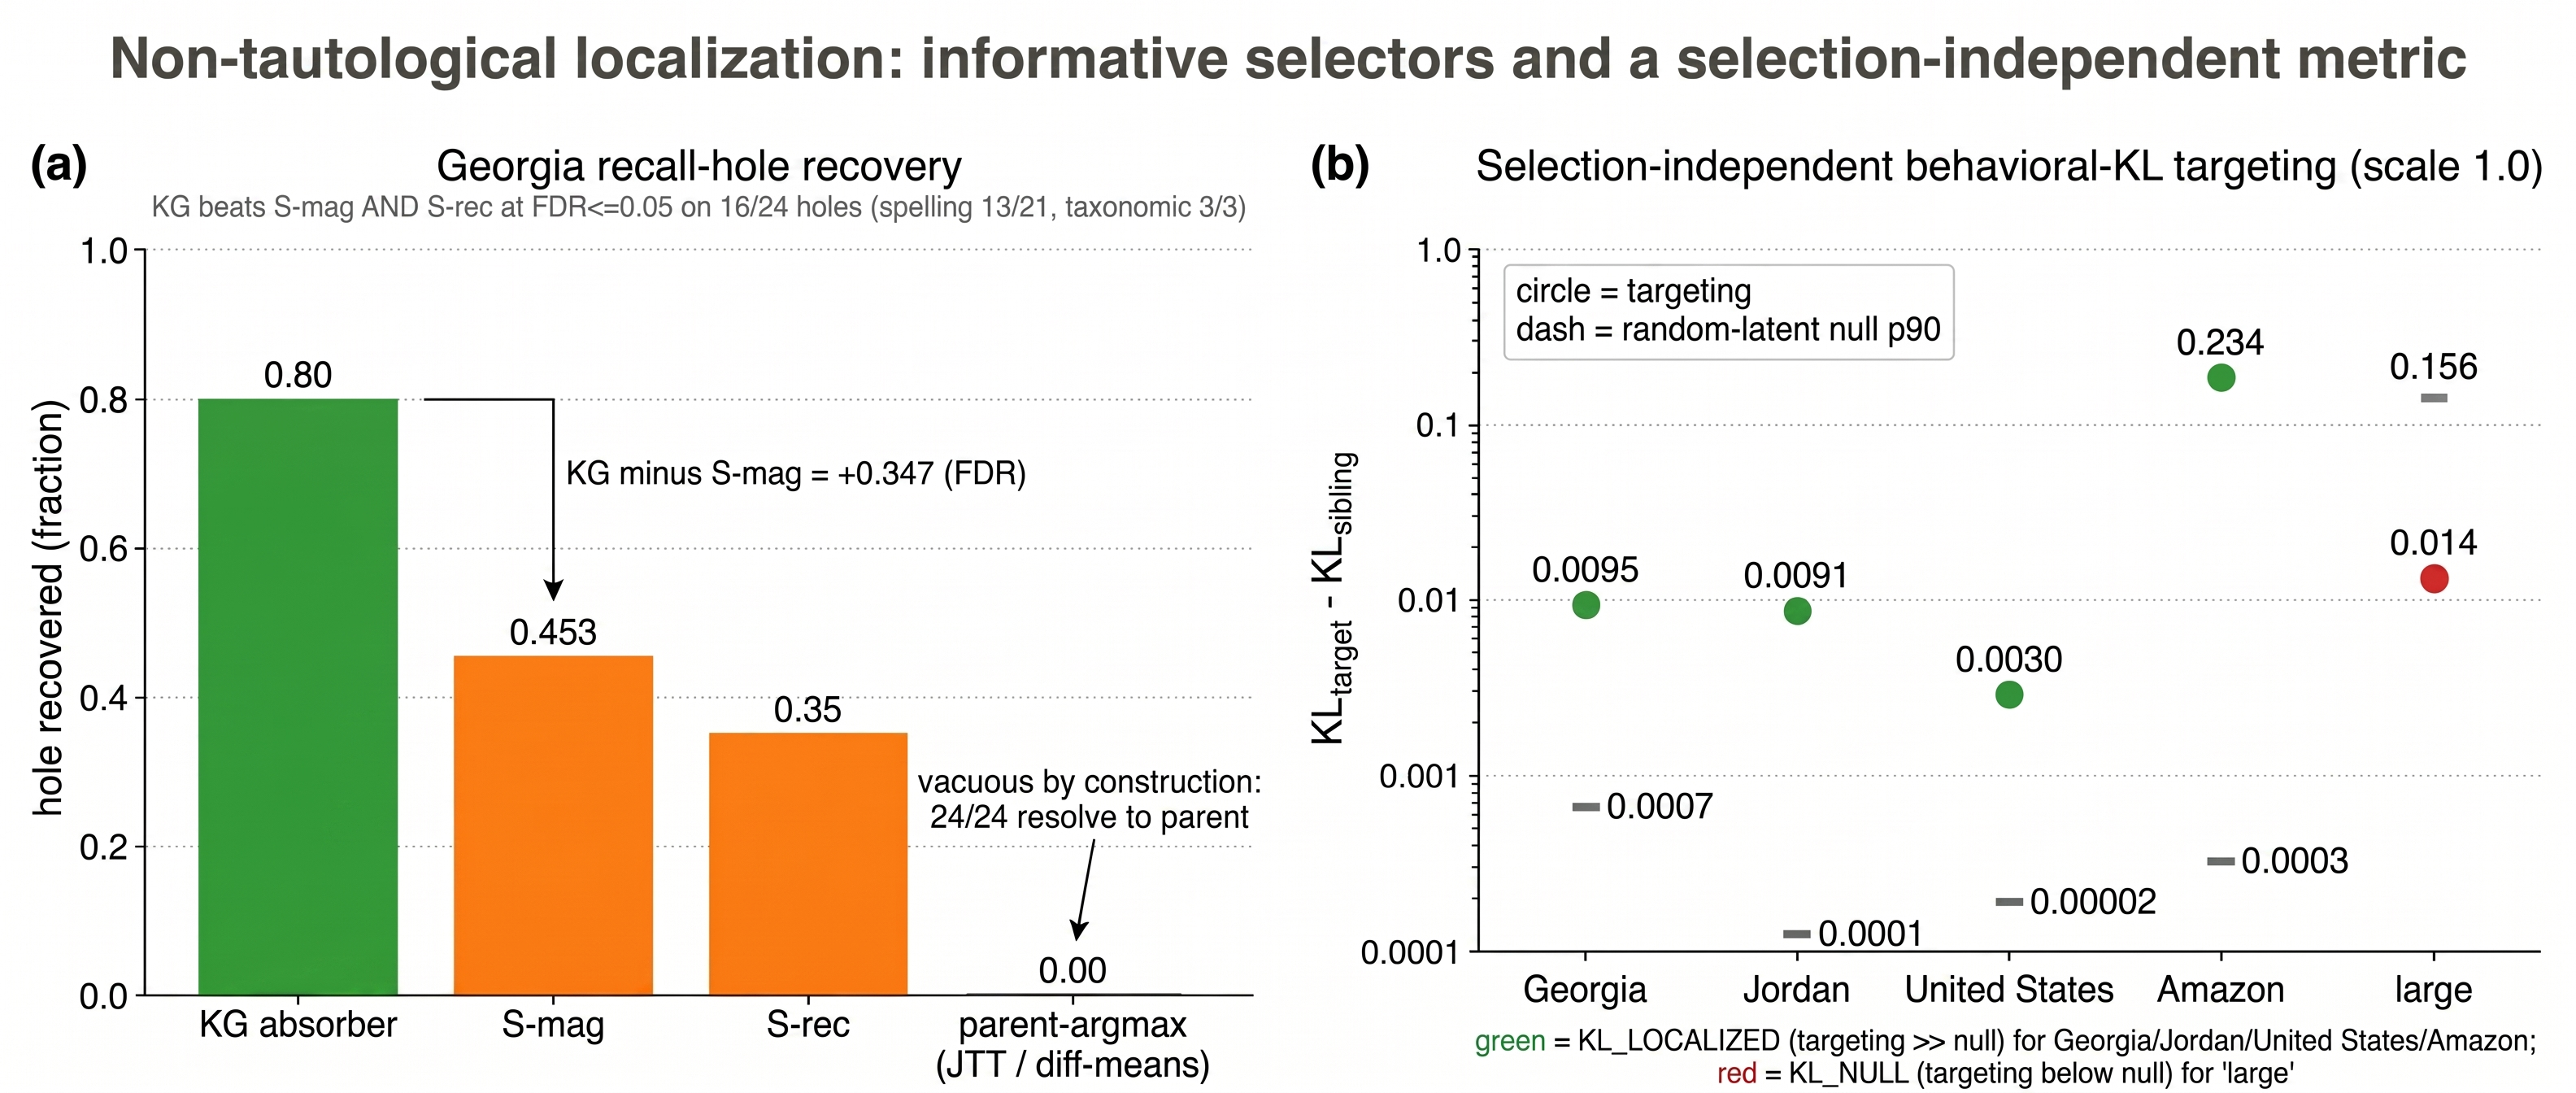
\includegraphics[width=\textwidth,height=0.45\textheight,keepaspectratio]{figures/fig3_v0.jpg}
  \caption{Left: Georgia recall-hole recovery for the KG-named absorber vs. the two informative label-free selectors S-mag and S-rec and the vacuous-by-construction parent-argmax controls (gain 0). Right: selection-independent next-token behavioral-KL targeting per case vs. a random-latent shuffle null; localized for Georgia/Jordan/US/Amazon, honestly null for `large'.}
  \label{fig:spine}
\end{figure*}

\paragraph{Coverage, not precision-magic, and non-trivial.} Within the same eligibility pool, ranking by per-sub-context precision is \emph{not} strictly better than ranking by magnitude or recall (\texttt{precision\_}\allowbreak\texttt{specific}$=$False): what matters is \emph{which} latent localizes the sub-context. The selectors are not strawmen: even label-free \textsc{S-mag} recovers $45.3\%$ of the Georgia hole, yet is beaten by $+0.347$ (FDR); and on $6/7$ numeric holes a stronger control matches-or-beats the KG, so the controls are genuinely non-trivial. The settled FDR family across the full repair loop has $30$ survivors over $24$ distinct holes (spelling $14$, taxonomic $6$, numeric $10$).

\paragraph{Selectivity is localization, not a surgical advantage.} The KG-named edit has $16$k absorption selectivity (on-target/collateral) of median $1262\times$, mean $1452\times$, with near-zero sibling collateral (mean $1.49\times10^{-4}$) and a $\sim0.4\%$ token footprint. We present this strictly as evidence the edit is \emph{localized}, because the selectivity denominator is the whole-parent erasure \textsc{Dense-Whole} (Table~\ref{tab:ops}), which over-shoots by construction. Against the \emph{genuinely fair} conditional control \textsc{Dense-Sub-Fair}, the surgical advantage disappears: on \texttt{large}, fair retain-collateral is $2.8\times10^{-6}$ vs.\ \textsc{KG-Abl}'s $5.1\times10^{-5}$ (the fair$-$KG collateral CI excludes $0$---the fair gate is significantly \emph{cleaner}). The residual win is over the strongest \emph{ungated} dense ($+0.97$ on \texttt{large}).

\paragraph{A selection-independent localization metric.} The localization-arm balanced accuracy is close to the firing-precision criterion the absorber was selected by, so its near-perfect value partly restates the selection. We therefore lean the claim on (i) held-out generalization to a disjoint eval fold and (ii) a selection-independent next-token behavioral-KL targeting metric the latent was \emph{not} chosen to optimize: the absorber's firing-gated ablation concentrates next-token KL on the sub-context relative to siblings, exceeding a random-latent shuffle null for Georgia ($0.0095$ vs.\ null $0.0007$), Jordan ($0.0091$ vs.\ $0.0001$), United States ($0.0030$ vs.\ $0.00002$), and Amazon ($0.234$ vs.\ $0.0003$). It is honestly \emph{null} for \texttt{large}, where a random content-responsive spelling latent dominates the null ($p_{90}{=}0.156>$ targeting $0.014$): firing-balanced-accuracy localizes that sense but behavioral-KL localizes only where the sense is lexically concentrated---an honest split we report rather than hide.

\paragraph{Members are auditable.} Describing each of $89$ unit members by its logit-lens top-$10$ tokens and top-$5$ activating windows with the sub-context label withheld, an ensemble LLM judge names the sub-context at agreement $0.730$ vs.\ a shuffle null of $0.096$ (gap $0.634$, CI $[0.545,0.724]$); absorbers are named at $0.756$, anchors at $0.429$ (the judge over-specifies the parent's mixed windows) \footnote{Code: \url{https://github.com/AMGrobelnik/ai-invention-7ee30c-catching-silent-feature-absorption-in-fr/tree/main/round-4/experiment-1}}.

\section{Where Absorption Hides: A Coverage Screen and a Cross-Dictionary Catalog}
\label{sec:catalog}

Absorption is a lexical-polysemy phenomenon---$6/110$ eligible polysemous tokens are structured, demographic safety attributes essentially never---and we ship both a label-free screen and a $1344$-row absorber catalog over a four-SAE public suite so the result is verifiable and reusable on any frozen SAE.

\paragraph{Coverage and confinement.} Across $10$ hierarchies, $336$ candidates screened, $110$ eligible, pooled strict coverage is $6/110=5.5\%$ (Wilson $[0.025,0.114]$); relaxed $31/336=9.2\%$. The $6$ strict-structured tokens are all homograph/named-entity (Table~\ref{tab:coverage}): Georgia (taxonomic; absorber $16009$), Amazon/Bush/Cook (named-entity; $6846$/$9751$/$15631$), and borderline British/Greek. Demographic religion ($0/10$), ethnicity ($0/10$), and calendar months ($0/12$) are never structured; professions $0/28$ (carried \footnote{Code: \url{https://github.com/AMGrobelnik/ai-invention-7ee30c-catching-silent-feature-absorption-in-fr/tree/main/round-5/experiment-4}}). A second \$$0$ screen over the full \texttt{civil\_comments} corpus ($1.76$M rows) finds exactly two of $44$ safety groups structured---\texttt{white} and \texttt{straight}, both homographs \footnote{Code: \url{https://github.com/AMGrobelnik/ai-invention-7ee30c-catching-silent-feature-absorption-in-fr/tree/main/round-6/experiment-2}}---and a named-entity pass finds $3/5$ \citep{Ahsan2025} \footnote{Code: \url{https://github.com/AMGrobelnik/ai-invention-7ee30c-catching-silent-feature-absorption-in-fr/tree/main/round-7/experiment-2}}. The form-free oracle corroborates $27/31$ structured candidates (lexical $26/29$); Georgia is the documented exception (decoder cosine $\approx0.01$), reported separately.

\paragraph{The catalog: a label-free feature-KG over a public suite.} We parametrize the shipped screen over four frozen Gemma-Scope SAEs---widths $\{16$k$,65$k$\}\times$ layers $\{9,12\}$---emitting one row per (candidate, config): $1344$ rows carrying the full firing signature, the predict-absorption verdict, the form-free oracle corroboration, anchor provenance, and a Neuronpedia auto-interp label for the parent and absorber latents ($203$ structured rows labeled, \$$0$). At $16$k/L12 the catalog reproduces our screen \emph{bit-exactly} ($336/336$ rows match on verdict and absorber id). Two dictionary laws emerge (Table~\ref{tab:catalog}, Figure~\ref{fig:catalog}): absorption is much more prevalent at the \emph{earlier} layer (strict-structured rises $6\to15$ at $16$k and $3\to29$ at $65$k going L12$\to$L9), and \emph{wider} SAEs surface more breadth (relaxed-structured $31\to62$ at L12, with $9/10$ hierarchies showing $65$k$\ge16$k)---directly consistent with ``wider absorbs more'' \citep{Karvonen2025, Chanin2025}. Absorber ids are dictionary-specific: of $131$ tokens structured in some config, only $8$ are persistent across $\ge3$ configs (Amazon and Jordan in all four), while $69$ are config-specific---so a latent's reliability must be checked \emph{per} SAE, which is exactly what the shipped screen and catalog enable.

\begin{figure*}[!t]
  \centering
  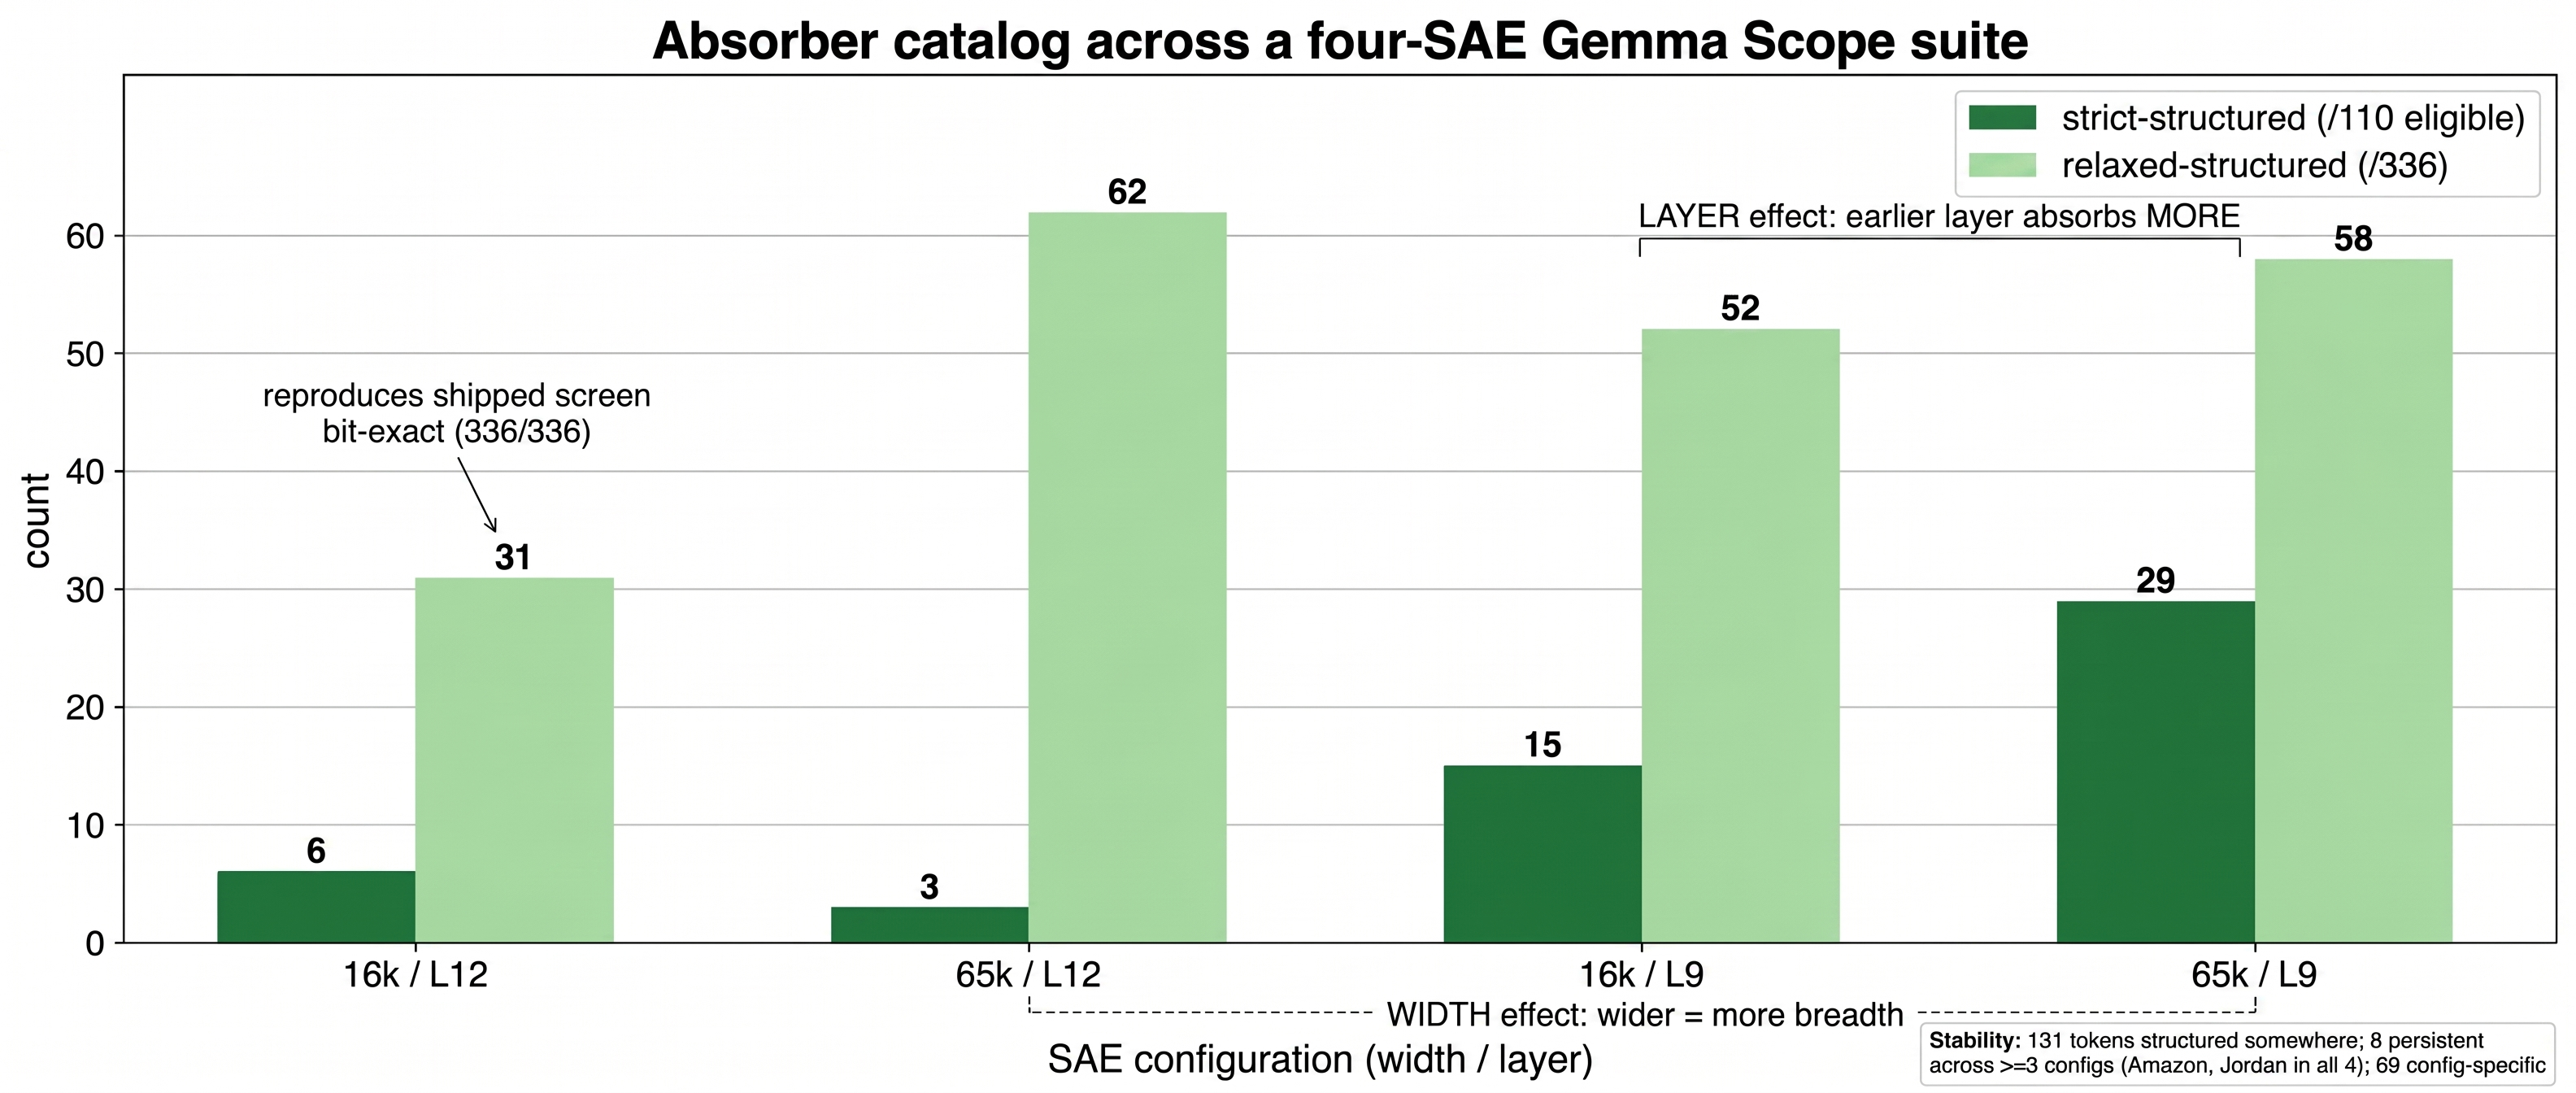
\includegraphics[width=\textwidth,height=0.45\textheight,keepaspectratio]{figures/fig4_v0.jpg}
  \caption{Absorption-structured counts across width $\{16$k$,65$k$\}$ and layer $\{9,12\}$. Absorption is far more prevalent at the earlier layer 9 (strict 6->15 at 16k, 3->29 at 65k going L12->L9) and wider at 65k (relaxed breadth). The 16k/L12 config reproduces the shipped screen bit-exactly (6/110 strict).}
  \label{fig:catalog}
\end{figure*}

\begin{table}[t]
\centering\small
\caption{Label-free coverage screen at $16$k/L12: \textsc{Absorption-Structured} count over eligible candidates. Absorption is homograph/named-entity-confined; demographic attributes are never structured. Pooled strict $6/110=5.5\%$ (Wilson $[0.025,0.114]$).}
\label{tab:coverage}
\begin{tabular}{lrrl}
\toprule
Hierarchy & eligible & struct. & structured tokens \\
\midrule
taxonomic country & $20$ & $1$ & Georgia (homograph) \\
named-entity & $5$ & $3$ & Amazon, Bush, Cook \\
nationality & $31$ & $2$ & British, Greek (homographs) \\
religion & $10$ & $0$ & --- \\
ethnicity & $10$ & $0$ & --- \\
homograph months & $12$ & $0$ & --- \\
homograph cities & $18$ & $0$ & --- \\
professions (carried) & $28$ & $0$ & --- \\
\midrule
\textbf{pooled (strict)} & \textbf{110} & \textbf{6} & all homograph/named-entity \\
\bottomrule
\end{tabular}
\end{table}

\begin{table}[t]
\centering\small
\caption{The absorber catalog across the four-SAE suite: \textsc{Absorption-Structured} counts (strict, $\ge150$ eligible) and breadth counts (relaxed). Absorption is far more prevalent at the earlier layer and wider at width $65$k. The $16$k/L12 column reproduces the shipped screen bit-exactly.}
\label{tab:catalog}
\begin{tabular}{lcccc}
\toprule
Config & strict$/110$ & relaxed$/336$ & avg.\ $L0$ & FVU \\
\midrule
$16$k / L12 (reproduces screen) & $6$ & $31$ & $82$ & $0.193$ \\
$65$k / L12 & $3$ & $62$ & $72$ & $0.170$ \\
$16$k / L9 & $15$ & $52$ & $73$ & $0.235$ \\
$65$k / L9 & $29$ & $58$ & $118$ & $0.166$ \\
\bottomrule
\end{tabular}
\end{table}

\paragraph{So what.} Because the field's own SAE-reliability proxies are contested and do not transfer \citep{Chanin2026}, a task-grounded, label-free, oracle-validated screen plus a published catalog is a transferable reliability instrument and a feature-level knowledge graph whose interventional recall-hole edges are invisible to observational co-occurrence/geometry KGs \citep{Winnicki2026}. Paired with the averted-cost demonstration (\S\ref{sec:averted}), the boundary statement ``absorption is confined'' becomes an actionable tool: an auditor can verify, label-free, that the demographic attributes they care about are co-firing---and where a homograph slice \emph{is} structured, name the absorber that repairs it.

\section{Genuine Cross-Deployment Where-to-Gate Transfer}
\label{sec:transfer}

A fixed absorber id discovered once on deployment $A$, applied with \emph{zero} new labels to a disjoint deployment $B$, beats a fresh $n$-label dense gate on $4/5$ sub-contexts, realizing a real per-redeployment label saving; one case is an honest no-transfer. This removes the circularity of a same-fold comparison: the dense gate is fit fresh on $B$'s own labels and \emph{both} gates are scored on a $B_{\text{eval}}$ disjoint from the $A$ discovery fold and from $B_{\text{fit}}$.

\paragraph{Protocol.} We discover the absorber id once on $A$ (the diagnostic fold), then on a disjoint deployment $B$ score the $n$-independent fixed-id SAE firing gate ($0$ deploy labels) against a fresh dense fair gate fit on $B$'s own $n$ labels ($n\in\{1,5,20,\text{full}\}$, $30$ resamples). $B$ is either a held-out corpus split ($B_{\text{fit}}/B_{\text{eval}}$ by a stable document hash) or a carrier shift (fit on templated pairs, deploy on natural corpus). Gate quality is balanced accuracy (TPR on held-out target-positive, TNR on sibling-positive).

\begin{figure*}[!t]
  \centering
  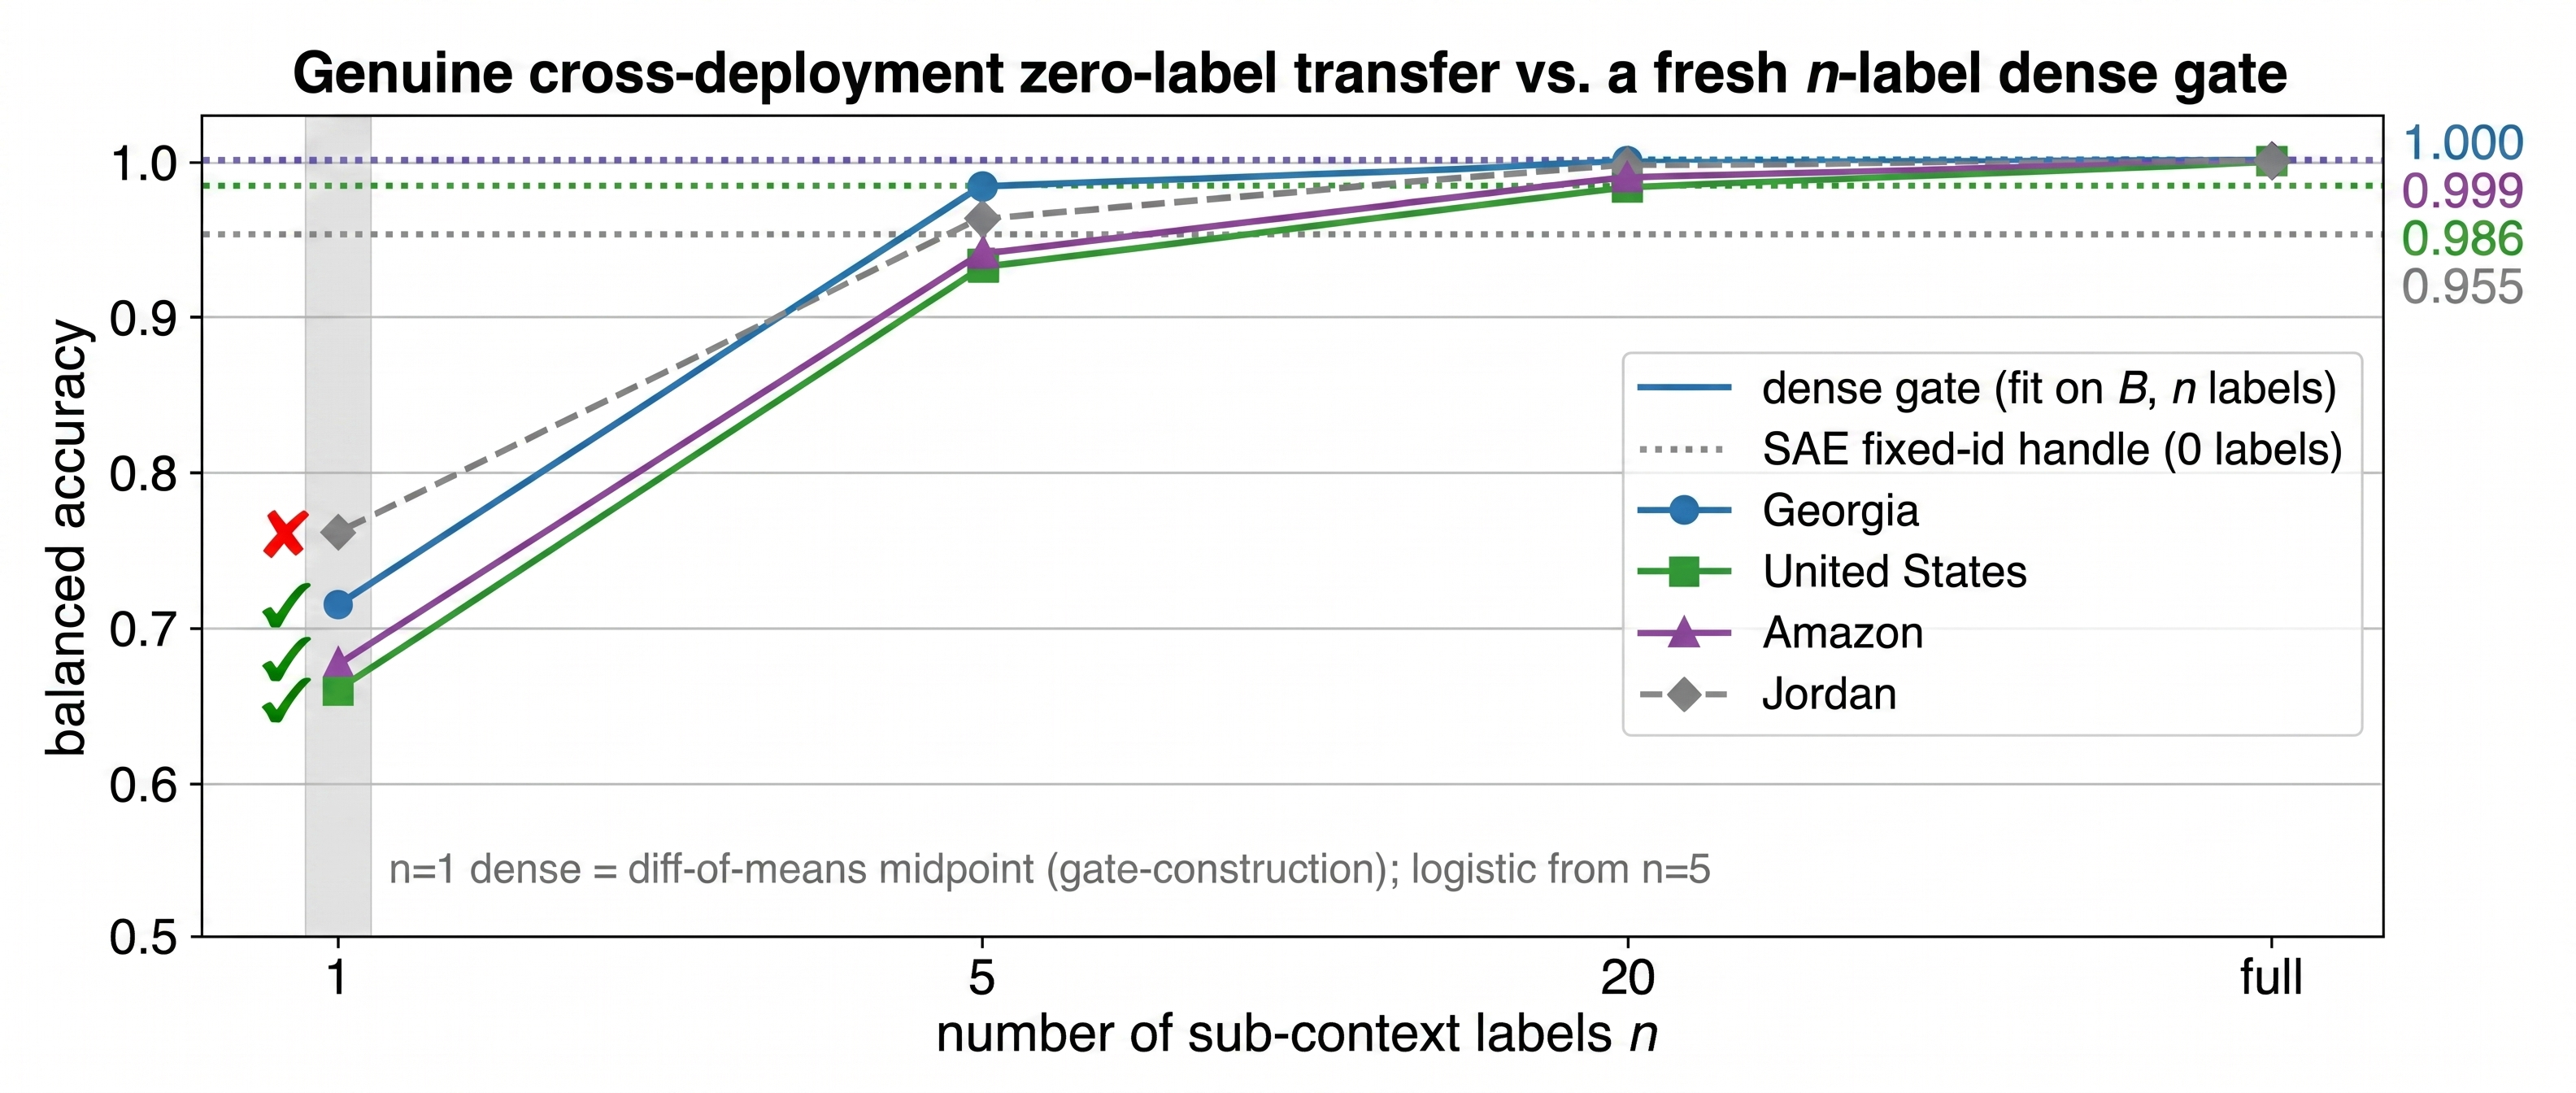
\includegraphics[width=\textwidth,height=0.45\textheight,keepaspectratio]{figures/fig5_v0.jpg}
  \caption{On a disjoint deployment B, the fixed-id SAE firing gate (0 deploy labels, horizontal lines) vs. a dense fair gate fit fresh on B's own n labels (rising curves). The handle beats the n=1 dense gate (CI-separated) for Georgia/US/Amazon; Jordan is an honest no-transfer (dense n=1 0.761 overlaps the 0.955 handle).}
  \label{fig:transfer}
\end{figure*}

\paragraph{Transfer is real on $4/5$ sub-contexts.} On the held-out corpus split (Table~\ref{tab:transfer}), the fixed-id SAE handle beats a fresh $n{=}1$ dense gate---with the dense CI separated below the handle---for Georgia (SAE $1.000$), United States ($0.986$), and Amazon ($0.999$); on the carrier shift the spelling case \texttt{large} also transfers ($0.995$ vs.\ dense $n{=}1$ $0.567$). Jordan is an honest \emph{no-transfer} case: the handle reaches only $0.955$, so a noisy $n{=}1$ dense gate's CI overlaps it. The honest practical comparison is the $n{=}5$ dense point, already within $\sim0.03$--$0.05$ of the SAE handle on the corpus-rich cases; the dramatic $n{=}1$ collapse is partly a gate-construction artifact, since the dense gate at $n{=}1$ is a diff-of-means midpoint and only becomes logistic at $n\ge5$.

\paragraph{Break-even and discovery cost, netted honestly.} The fixed-id handle uses zero labels \emph{at deployment} but pays a one-time discovery cost $D$ on $A$; we report the break-even $K^\star=D/n^\star$ (redeployments to amortize against an $n^\star$-label dense gate refit each time): Georgia $K^\star{=}150$, United States $600$, Amazon $\approx70$. We also ask whether the absorber id is cheaply re-discoverable from few labels: it is for Jordan ($20$) and \texttt{large} ($10$), but \emph{not} for Georgia/US/Amazon, where a label-frugal re-derivation picks a weaker split sibling---an honest feature-splitting signal that makes the catalog's pre-computed id the load-bearing value for those cases. The decisive evidence is the low-$n$ CI separation on a genuine deployment $B$, not the amortized $K^\star$. The same-fold $A$ contrast reproduces our prior numbers exactly, confirming that the only change is the non-circular $B$ deployment.

\begin{table}[t]
\centering\small
\caption{Cross-deployment transfer on a disjoint corpus split $B$. The fixed-id SAE handle ($0$ deploy labels) vs.\ a fresh dense gate fit on $B$'s own $n$ labels (balanced accuracy). The handle beats $n{=}1$ dense (CI-separated) for Georgia/US/Amazon; Jordan is an honest no-transfer; \texttt{large} is underpowered on $B$ but transfers on the carrier shift. $K^\star{=}D/n^\star$ is the break-even redeployment count.}
\label{tab:transfer}
\begin{tabular}{lcccccll}
\toprule
& SAE & \multicolumn{4}{c}{dense gate @ $n$ labels} & & \\
\cmidrule(lr){3-6}
Case & handle & $1$ & $5$ & $20$ & full & $K^\star$ & verdict \\
\midrule
Georgia & $1.000$ & $0.718$ & $0.983$ & $0.999$ & $1.000$ & $150$ & confirmed \\
United States & $0.986$ & $0.664$ & $0.936$ & $0.984$ & $1.000$ & $600$ & confirmed \\
Amazon & $0.999$ & $0.674$ & $0.940$ & $0.990$ & $1.000$ & $70$ & confirmed \\
Jordan & $0.955$ & $0.761$ & $0.964$ & $0.990$ & $1.000$ & --- & no-transfer \\
\texttt{large}$^\ddagger$ & $0.991$ & $0.630$ & $0.916$ & $0.983$ & $0.999$ & --- & (carrier shift) \\
\bottomrule
\end{tabular}
\\[2pt]
{\footnotesize $^\ddagger$ underpowered on $B$ ($7$ eval positives); transfer confirmed on the carrier-shift axis (SAE $0.995$ vs.\ $n{=}1$ dense $0.567$).}
\end{table}

\paragraph{The Amazon edit caveat, substantiated.} The transfer experiment also diagnoses the one load-bearing caveat directly. On the Amazon \emph{edit} arm, at matched behavioral forget the judge-measured forget gap between the SAE handle and the fair dense gate is $0.875$ (CI $[0.25,1.5]$, $>0.3$ materiality), so the two routes do \emph{not} forget equally at the matched point. We therefore report both metrics: the preservation-at-matched-forget advantage \texttt{adv\_pres} is $0.000$ at full labels (CI includes $0$) and $+0.911$ at $n{=}1$, while the stricter joint \texttt{adv\_joint} stays $+0.523$ at full labels as an instrument-disagreement artifact (the judge scores the SAE handle forgetting more), not a label-scarcity effect. For Amazon we therefore soften the edit claim to a \emph{preservation-advantage-only} result. The \texttt{large} arm has an isolated, immaterial offset (both routes forget well, residual gap $0.0$), so its preservation advantage stands.

\section{What Did Not Pay Off, Reported Honestly}
\label{sec:nulls}

The clustering hypothesis and all three goal-named downstream tasks are nulls; we report each with its statistic.

\paragraph{The clustering hypothesis is inert.} Replacing the anchored set-cover with the single most precise latent ties \textsc{KG-Abl} on every edit ($0/8$ cases the machinery adds value; $3/8$ it returns the \emph{same} latent); ablating the multi-member unit instead of the single absorber strictly lowers retained utility (\texttt{large}: single $1.87$ vs.\ unit $1.38$) \footnote{Code: \url{https://github.com/AMGrobelnik/ai-invention-7ee30c-catching-silent-feature-absorption-in-fr/tree/main/round-6/experiment-1}}; and the correlation-community track ties weak baselines (toxicity unit AUC $0.762$ vs.\ best raw latent $0.765$). What discovery buys over max-precision is solely the recall-hole \emph{anchoring} that names \emph{which} sub-context to gate.

\paragraph{The three goal-named tasks are nulls.} (1) \emph{Classification}: no SAE unit out-classifies a dense probe (Georgia $0.995$ vs.\ $1.000$; toxicity unit AUC $0.762$ vs.\ dense $0.84$--$0.89$; sub-attributes $0.63$ vs.\ $0.93$)---consistent with the downstream-capability null where the repaired unit does not out-recall a dense probe on $4/5$ concepts (the value is auditable localization, a handle the dense hyperplane lacks). (2) \emph{Steering}: the unit's mean-member direction is most surgical only on letters L and D ($2/5$) \footnote{Code: \url{https://github.com/AMGrobelnik/ai-invention-7ee30c-catching-silent-feature-absorption-in-fr/tree/main/round-2/experiment-1}}. (3) \emph{Model-diffing}: no instruction-tuned Gemma Scope 2B SAE exists, so the shared-SAE base-vs-IT shift is detectable but not concept-specific (control-subtracted shift $+0.000$, CI $[-0.009,0.007]$) \footnote{Code: \url{https://github.com/AMGrobelnik/ai-invention-7ee30c-catching-silent-feature-absorption-in-fr/tree/main/round-3/experiment-5}}.

\paragraph{The edit, as an edit, has no SAE-specific advantage.} A genuinely fair $d_{\text{sub}}$-gated dense control matches the discovered absorber at full labels and is cleaner on collateral; gating is prior art \citep{Lee2024, Zhang2026, Turani2026, Wang2024}. The residual win over the strongest \emph{ungated} dense ($+0.97$ on \texttt{large}, $+0.87$ on \texttt{Amazon}) tracks lexical \emph{concentration} (point-biserial $r{=}{+}0.63$), not the absorption label ($r{=}{-}0.09$) \footnote{Code: \url{https://github.com/AMGrobelnik/ai-invention-7ee30c-catching-silent-feature-absorption-in-fr/tree/main/round-8/evaluation-1}}; a concentrated co-firing latent (\texttt{insult}) forgets while distributed absorbers (Georgia/Jordan) do not. The recall-hole \emph{router} reproduces on derivation (balanced accuracy $1.0$) but its prospective stratum has Wilson CIs including $0.5$, so it is demoted to an exploratory diagnostic.

\section{Discussion}
\label{sec:discussion}

\paragraph{What is established.} On a frozen Gemma Scope SAE, label-free single-specialist localization surfaces the absorber that marginal attribution drops and emits an auditable feature KG and a published cross-dictionary catalog with measured, localized recall recovery that beats the informative label-free selectors and replicates at $4\times$ width. The reliability gain is \emph{localization and auditability}, not classification. The build-on capability is the \emph{averted-cost} pairing: a practitioner who ships a compact SCR/TPP classifier/steerer silently fails on an absorbed slice, standard tooling misses it, the shipped screen catches it, and the named-absorber two-member unit repairs it---and where the saving is label-free, a fixed absorber id transfers zero-label to a disjoint deployment and beats an $n$-label dense gate on $4/5$ sub-contexts.

\paragraph{A regime-scoped contribution with an explicit ``so what.''} The regime where the localization adds value---homograph-polysemy absorption with a suppressed parent---is narrow ($6/110$ eligible tokens) and does not coincide with the demographic safety attributes one might first audit. We turn this into a contribution: absorption-reliability is a lexical-polysemy phenomenon, so an auditor can verify label-free that demographic attributes are co-firing and need not fear absorption there, while the catalog names the absorbers for the homograph/named-entity slices that \emph{are} structured.

\paragraph{Limitations.} (i) The clustering machinery is inert; the durable object is a single specialist plus a two-member repair unit. (ii) No SAE unit out-classifies a dense probe; the edit is matched by a fair labeled gate, and the Amazon edit arm is softened to preservation-advantage-only. (iii) The structure is homograph-confined; demographic safety attributes are essentially never absorption-structured. (iv) The transfer saving is genuine but de-inflated ($4/5$; one no-transfer; large $K^\star$ for the feature-split cases). (v) Replication is layer-conditional and numeric is below the editing gate (digit-token cosine $0.876$--$0.891<0.9$). (vi) Model-diffing is infrastructure-bounded. Each is a measured finding with its statistic, not a deferral.

\section{Conclusion}
\label{sec:conclusion}

We set out to cluster frozen-SAE latents into more reliable units and found that the clustering hypothesis does not pay off; what does is \emph{label-free single-specialist localization}---anchor on the highest-recall parent, read its recall hole to name an under-served sub-context with no sub-context labels, and precision-select the single absorber that marginal attribution drops. We convert this from a reassurance into a capability: on a compact classifier/steerer the standard practice ships, absorption silently breaks the absorbed slice (Georgia recall $0.107$ vs.\ $0.969$), standard tooling misses the absorber (rank $42$, oracle blind), the shipped label-free screen catches and names it, and a two-member repair unit recovers recall to $\approx1.0$ and the steer by $+5.74$. The where-to-gate saving is real and de-inflated: a fixed absorber id transfers zero-label to a disjoint deployment and beats an $n$-label dense gate on $4/5$ sub-contexts. We ship the screen and a $1344$-row absorber catalog over four public SAEs. The honest ceiling stands---no SAE unit out-classifies a dense probe and the edit is matched by a fair labeled gate---but \emph{finding where to act, and what it would silently cost you, is label-free, auditable, and verifiable on any frozen SAE}.

\paragraph{Future work.} Characterize a priori what makes an absorbed feature concentrated enough to edit; extend the catalog to more SAE suites and to Neuronpedia at scale; mine wider vocabularies for additional concentrated suppressed-parent homographs; and revisit model-diffing if a paired instruction-tuned SAE becomes available.

\appendix
\section{Appendix: Changelog, Selectors, and Reproducibility}
\label{sec:appendix}

\paragraph{Changelog (self-corrections folded here).} The body presents corrected results as the results. For transparency: a prior version of this work reported a label-scarce ``where-to-gate'' saving in which the SAE handle's absorber id had been discovered with full sub-context labels while only the dense gate was restricted to $n$ labels; \S\ref{sec:transfer} replaces that same-fold comparison with a genuine cross-deployment transfer (fixed id, zero deploy labels, disjoint $B_{\text{eval}}$) and reports the break-even $K^\star$ and an honest no-transfer case. A prior version also claimed a $+1.58$ edit win over a footprint-matched gate; that gate was mis-tuned ($\beta\approx3.0$, $14\times$ over-erasure), the defensible lead is $+1.00$ (CI $[0.79,1.21]$) over the strongest \emph{ungated} dense, and a genuinely fair conditional gate closes even that gap. A prior Georgia ``$+0.561$'' edit win is retracted as near-NOOP. Selectivity is now presented strictly as localization (the whole-parent denominator is the disowned strawman), the $65$k selectivity is reported as the corrected median $\sim676\times$ (never the $466997\times$ divide-by-$\epsilon$ artifact), and the four-control framing is reframed: the win is over the two informative label-free selectors \textsc{S-mag}/\textsc{S-rec}, with the parent-argmax controls reported as vacuous-by-construction.

\paragraph{Selector zoo (relegated).} The label-free count-matched selectors \textsc{S-rec} (top-$k$ by recall), \textsc{S-prec} (by precision), and \textsc{S-mag} (by magnitude), the random-eligible-$k$ floor, and the supervised oracle pools are used only to isolate the selection rule; within-SAE precision-gated selection on Georgia reaches AUC $0.995$, beating every label-free selector with CIs excluding $0$ \footnote{Code: \url{https://github.com/AMGrobelnik/ai-invention-7ee30c-catching-silent-feature-absorption-in-fr/tree/main/round-4/experiment-3}}.

\paragraph{Encoding and software.} SAEs load from Gemma Scope \texttt{params.npz} (primary canonical \texttt{layer\_12/}\allowbreak\texttt{width\_16k}, \texttt{average\_l0\_82}, JumpReLU, $d_{\text{model}}{=}2304$; suite \texttt{width\_65k} and \texttt{layer\_9}); residual via a forward hook on \texttt{model.layers[L]} (\texttt{hidden\_states}[$L{+}1$], chosen by min-FVU). Gating cosine $0.919$ ($16$k), $0.928$ ($65$k); numeric digit-token cosine $0.876$--$0.891$, flagged below-gate. Model \texttt{google/gemma-2-2b} (and \texttt{-2b-it} for model-diffing) via ungated mirrors, bf16. The averted-cost, transfer, screen, and catalog experiments reuse the surgical-edit engine verbatim and add the SCR/TPP selection harness, the catalog driver, and two LLM judges (\texttt{claude-haiku-4.5} primary, \texttt{gpt-4o-mini} second). Total LLM spend across the new experiments was under \$$0.07$ (the averted-cost judge \$$0.01$, the transfer judges \$$0.05$); the screen and catalog cost \$$0$; all compute is on a single $12$--$23$GB GPU. Citation venues follow a verified audit (e.g.\ \citet{Chanin2024} NeurIPS 2025; \citet{Wu2025}, \citet{Karvonen2025}, \citet{Gallifant2025} 2025 venues; \citet{Leask2025}, \citet{Lee2024}, \citet{Marks2024} ICLR 2025).

\bibliographystyle{plainnat}
\bibliography{references}

\end{document}
